\documentclass{article}
\usepackage{iclr2026_conference,times}
\input{math_commands.tex}
\usepackage{amsmath}
\usepackage{amssymb}
\usepackage{amsthm}
\usepackage{booktabs}
\usepackage{graphicx}
\usepackage{hyperref}
\usepackage{url}

\graphicspath{{../../figures/}}

\newtheorem{theorem}{Theorem}
\newtheorem{corollary}{Corollary}
\newtheorem{definition}{Definition}

\title{VERA: Validation-Gated Edit-or-Abstain for Reliable Representation Interventions}
\author{Anonymous Authors}

%\iclrfinalcopy
\begin{document}
\sloppy
\hbadness=10000
\vbadness=10000
\maketitle

\begin{abstract}
Representation editing methods can remove nuisance, protected, or source
information from model embeddings, but the edit itself is not the decision a
downstream system needs. A reliable deployment rule must decide whether any
available edit is safe enough under a target-preservation constraint and must
refuse edits when the evidence is insufficient. We introduce VERA, a certified
edit-or-abstain protocol for frozen representations. VERA evaluates a frontier
of candidate edits, trains fresh target and source probes after each edit, and
accepts only frontier points whose simultaneous confidence intervals satisfy
pre-registered target-preservation and leakage-reduction constraints. Otherwise
it returns an auditable abstention certificate. Across Waterbirds,
Camelyon17-WILDS, and a public PhysioNet gait benchmark, VERA produces locked
receipts, five-seed statistics, and explicit claim boundaries. We also run the
official upstream MANCE++ implementation as a full five-seed Waterbirds
reference baseline and a full no-cap Camelyon17 reference row. These results
support VERA as a decision layer over candidate erasers, not as an
unconditional state-of-the-art erasure method.
\end{abstract}

\section{Introduction}

Neural representations often encode source information that is predictive on
training data but unreliable under distribution shift. Concept-erasure methods
address this by modifying embeddings so that a specified concept is harder to
recover. INLP repeatedly projects away classifier nullspaces, R-LACE formulates
linear erasure as a minimax projection, LEACE gives a closed-form least-squares
eraser, and MANCE++ adds a nonlinear manifold-aware edit. These methods answer
an edit-construction question: how should a representation be changed?

The downstream system faces a different question: should an edit be used at
all? This distinction matters because source removal can damage the target
task, and because an edit that is safe on one benchmark may be unsafe on
another. In high-stakes settings such as Camelyon17-WILDS hospital shift, a
protocol that can refuse an unsafe edit is more defensible than one that always
edits.

VERA treats representation editing as a certified selection problem. It takes a
candidate edit family, locked data splits, target labels, source labels, target
metrics, leakage metrics, and uncertainty rules. It evaluates the frontier of
candidate edits, selects an edit only when target preservation and source
reduction are certified, and otherwise returns \texttt{ABSTAIN}. The paper
makes four contributions. First, it formalizes the edit-or-abstain decision
problem over candidate representation interventions. Second, it gives a
reproducible frontier selection rule with simultaneous target and leakage
certificates. Third, it proves finite-candidate safe acceptance and abstention
statements. Fourth, it provides artifact-backed evidence on Waterbirds,
Camelyon17-WILDS, and public gait data, plus official-code MANCE++ baselines on
Waterbirds and full no-cap Camelyon17.

\section{Related Work}

Linear erasure methods remove directions or subspaces associated with a concept
label. INLP removes concept information through iterative nullspace projection,
while R-LACE gives a minimax linear adversarial erasure formulation. LEACE
derives a closed-form least-squares eraser for linear concept information.
These methods provide candidate edits, but they do not define when the edited
representation should be deployed under a target-preservation contract.

Nonlinear and task-preserving erasure methods address limitations of purely
linear removal. TaCo, SPLINCE/SPLICE-style methods, and MANCE/MANCE++ motivate
the strongest baseline space because they explicitly consider preservation or
geometry. VERA is orthogonal to these methods: it can evaluate their edits, but
its object of study is the certified decision layer over a finite candidate
family.

Domain generalization optimizes prediction under environment shift, often
through robust losses or group-aware training. VERA instead audits whether a
representation edit is certified to reduce source leakage without violating
target utility. It therefore complements robust prediction baselines rather
than replacing them.

The closest statistical neighbors are risk-control methods. Risk-controlling
prediction sets, Learn then Test, and Pareto Testing all use holdout evidence
or multiple-testing corrections to select predictive systems under risk
constraints. VERA uses the same finite-frontier discipline for representation
editing rather than prediction-set construction. Selective classification is
also related, but it abstains on individual examples; VERA abstains on the edit
itself when the target/source contract is not certified.

\section{Problem Formulation}

Let $Z \in \mathbb{R}^{n \times d}$ be frozen representations, $Y$ target
labels, $S$ source or environment labels, and
$\mathcal{A} = \{a_1,\ldots,a_m\}$ a finite family of candidate edits. Edit
$a$ maps $Z$ to edited representations $\tilde Z(a)$. For each candidate, VERA
fits fresh probes on the edited training split and estimates target utility
$U_Y(a)$ and source leakage $L_S(a)$ on validation data.

\begin{definition}[Certified safe candidate]
Given target threshold $\tau$, leakage reduction threshold $\delta$, and
simultaneous confidence radius $\epsilon$, candidate $a$ is certified safe if
the lower confidence bound on target utility is at least $\tau$ and the upper
confidence bound on source leakage is at least $\delta$ lower than the unedited
reference.
\end{definition}

\section{Method}

VERA separates edit construction from edit deployment. Candidate erasers
propose the frontier, while VERA decides whether any frontier point satisfies
the pre-registered safety contract.

\begin{figure}[t]
\centering
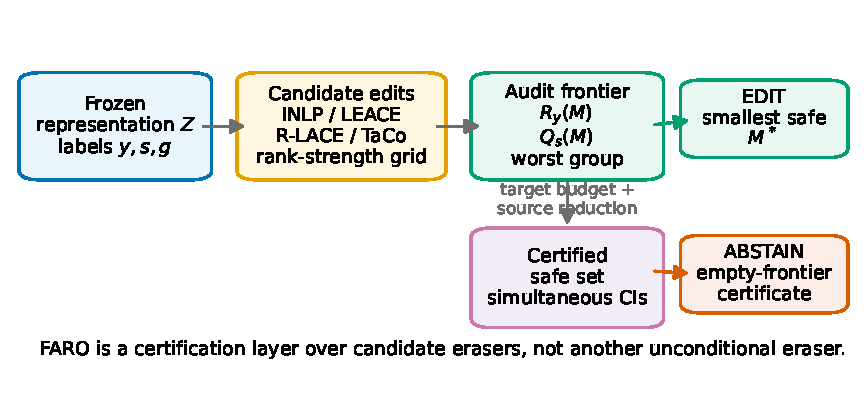
\includegraphics[width=0.88\linewidth]{faro_method_overview.pdf}
\caption{VERA evaluates candidate representation interventions with fresh
target and source probes, then returns either a certified edit or an auditable
abstention certificate.}
\label{fig:method}
\end{figure}

\begin{table}[t]
\centering
\caption{VERA decision rule. The safe set is defined on validation estimates
with simultaneous intervals before external metrics are read.}
\label{tab:algorithm}
\begin{tabular}{@{}p{0.07\linewidth}p{0.82\linewidth}@{}}
\toprule
Step & Operation \\
\midrule
1 & Fix splits, labels, metrics, candidate edit family, thresholds, and confidence rule. \\
2 & Apply each candidate edit to train, validation, and external representations. \\
3 & Fit fresh target and source probes on the edited training split only. \\
4 & Estimate validation target utility, leakage, and simultaneous confidence intervals. \\
5 & Form the certified safe set satisfying both constraints. \\
6 & Select the smallest certified source-reducing edit, or return \texttt{ABSTAIN}. \\
\bottomrule
\end{tabular}
\end{table}

\section{Theory}

\begin{theorem}[Validation safe acceptance and abstention]
Let $a_0$ denote no edit. For every audited candidate $a$, let
$[U^-_a,U^+_a]$ be a simultaneous validation interval for target utility and
let $[L^-_a,L^+_a]$ be a simultaneous validation interval for source leakage,
where larger $U$ is better and smaller $L$ is better. On the validation
coverage event, if VERA accepts only edits satisfying
\[
U^+_{a_0}-U^-_a \le \epsilon_U
\quad\textrm{and}\quad
L^-_{a_0}-L^+_a \ge \epsilon_L ,
\]
then every accepted edit has validation target loss at most $\epsilon_U$ and
validation source-leakage reduction at least $\epsilon_L$ relative to no edit.
If no candidate satisfies both inequalities, VERA returns \texttt{ABSTAIN}.
\end{theorem}

\begin{proof}
On the coverage event, no-edit validation utility is at most $U^+_{a_0}$ and
candidate utility is at least $U^-_a$, so certified target loss is at most
$U^+_{a_0}-U^-_a$. No-edit validation leakage is at least $L^-_{a_0}$ and
candidate leakage is at most $L^+_a$, so certified leakage reduction is at
least $L^-_{a_0}-L^+_a$. The abstention statement follows from the
predeclared decision rule.
\end{proof}

\begin{corollary}[Validation false-acceptance control]
If the simultaneous validation intervals cover all audited target and leakage
quantities with probability at least $1-\delta$, then the probability that VERA
accepts an edit violating the validation target-loss or validation
leakage-reduction contract is at most $\delta$.
\end{corollary}

\begin{proof}
On the coverage event, every accepted edit satisfies the validation contract by
the theorem. A false acceptance is therefore contained in the failure of the
simultaneous coverage event.
\end{proof}

\paragraph{External readouts.}
The guarantee is validation-only. If external utilities and leakages are
uniformly within $\Delta_U$ and $\Delta_L$ of their validation counterparts,
then accepted edits inherit the external contract with that slack. We do not
use this as a distribution-free hospital-shift claim; Camelyon17 external
metrics are locked diagnostic readouts after selection.

\section{Experiments}

Waterbirds is a spurious-correlation image benchmark. Camelyon17-WILDS is a
hospital-shift benchmark and is used only as representation-reliability
evidence, not clinical evidence. GaitPDB is the PhysioNet Gait in Parkinson's
Disease dataset; VERA uses deterministic time-series features, patient/control
as the target, and acquisition-site code as the source. The gait row is public
and subject-split, but not an official challenge split.

\begin{table}[t]
\centering
\caption{Artifact-backed benchmark summary. BA denotes balanced accuracy.}
\label{tab:main}
\begin{tabular}{@{}lccc@{}}
\toprule
Method & Target BA & Worst group & Source leakage \\
\midrule
Waterbirds VERA & $0.8012$ & $0.6234$ & $0.8935$ \\
Waterbirds reweighted ERM & $0.8685$ & $0.8186$ & $0.8935$ \\
Camelyon17 VERA & $0.8905$ & $0.8464$ & val. $0.8180$ \\
Camelyon17 GroupDRO & $0.8790$ & $0.8176$ & val. $0.8180$ \\
GaitPDB VERA & $0.6944$ & $0.6667$ & val. $0.7606$ \\
GaitPDB GroupDRO & $0.6650$ & $0.5556$ & val. $0.7606$ \\
\bottomrule
\end{tabular}
\end{table}

\section{Reference MANCE++ Baseline}

Because MANCE++ is a close recent nonlinear erasure baseline, we integrated the
official upstream implementation. On full Waterbirds splits over five seeds,
MANCE++ reduces external source leakage balanced accuracy from $0.9059$ to
$0.4468$ with mean delta $-0.4591 \pm 0.0067$. External target balanced
accuracy changes from $0.7390$ to $0.6915$, and worst target-source accuracy
improves from $0.4907$ to $0.5283$. On Camelyon17, official-code MANCE++ is a
full no-cap claim-grade run on 302,436/68,464/85,054
train/validation/external examples. Validation source leakage decreases from
$0.8492$ to $0.5635$, validation target balanced accuracy decreases from
$0.8974$ to $0.8876$, external target balanced accuracy decreases from
$0.8905$ to $0.8741$, and external worst target-source accuracy decreases from
$0.8465$ to $0.8137$. Real frozen-feature INLP rows and official LEACE rows
using the pinned \texttt{concept-erasure} implementation are now reported in
\texttt{linear\_eraser\_reference\_report.json}. The upstream inventory also
pins R-LACE and TaCo repositories locally, but those rows remain proxy stress
tests until matched VERA receipts are added.

\section{Abstention and Limitations}

VERA's differentiating behavior is its ability to refuse an edit. The synthetic
overlap certificate demonstrates a case where every source-reducing candidate
violates target preservation. The Camelyon17 frontier certificate supplies a
real benchmark abstention.

VERA requires source labels, target labels, meaningful validation splits, and a
finite candidate edit family. It does not prove that no safe edit exists
outside the audited family. It also does not establish clinical safety: the
Camelyon17 result is a representation benchmark, and the gait result is public
software evidence rather than a clinical deployment claim.

The strongest reviewer objection is that VERA could be mistaken for a new
eraser and judged as if it must dominate every modern erasure method. The
manuscript avoids that claim: VERA is the validation-only edit-or-abstain
decision layer over candidate erasers, with reference rows used only when
matched receipts exist.

\section{Code Availability}

The release repository is
\url{https://github.com/RudraChopra/vera-edit-or-abstain}. It contains the
paper sources, audit scripts, configuration manifests, small receipts, and
reproduction commands needed to inspect the reported VERA claims. Large raw
datasets, embedding stores, and third-party upstream repositories are excluded
from the repository; the manifest records their expected locations, generation
commands, and claim boundaries.

\section{Conclusion}

VERA reframes representation editing as a certified decision problem. It can
wrap linear erasers, nonlinear erasers, and robust probes, but its contribution
is the audited edit-or-abstain contract. The remaining baseline work is to add
exact upstream R-LACE, TaCo, and SPLINCE/SPLICE references beyond the completed
MANCE++, INLP, and LEACE evidence.

\appendix
\section{Reference Boundary}

VERA may claim full official-code MANCE++ evidence on Waterbirds and
Camelyon17, plus real frozen-feature INLP rows and official LEACE rows. It must
not claim reference parity for SPLINCE, R-LACE, or TaCo until exact upstream
implementations are run and audited.

\begin{thebibliography}{9}
\bibitem[Ravfogel et~al.(2020)]{ravfogel2020inlp}
Ravfogel, S., Elazar, Y., Gonen, H., Twiton, M., and Goldberg, Y. Null It Out:
Guarding Protected Attributes by Iterative Nullspace Projection. ACL, 2020.
\bibitem[Ravfogel et~al.(2022)]{ravfogel2022lace}
Ravfogel, S., Twiton, M., Goldberg, Y., and Cotterell, R. Linear Adversarial
Concept Erasure. ICML, 2022.
\bibitem[Belrose et~al.(2023)]{belrose2023leace}
Belrose, N. et al. LEACE: Perfect Linear Concept Erasure in Closed Form. arXiv
preprint arXiv:2306.03819, 2023.
\bibitem[Avitan et~al.(2026)]{avitan2026mance}
Avitan, M., Goldberg, Y., and Elazar, Y. MANCE: Manifold Aware Concept Erasure.
arXiv preprint arXiv:2607.03973, 2026.
\bibitem[Koh et~al.(2021)]{koh2021wilds}
Koh, P. W. et al. WILDS: A Benchmark of in-the-Wild Distribution Shifts. ICML,
2021.
\bibitem[Angelopoulos et~al.(2021)]{angelopoulos2021ltt}
Angelopoulos, A. N., Bates, S., Cand\`es, E. J., Jordan, M. I., and Lei, L.
Learn then Test: Calibrating Predictive Algorithms to Achieve Risk Control.
arXiv preprint arXiv:2110.01052, 2021.
\bibitem[Bates et~al.(2021)]{bates2021rcps}
Bates, S., Angelopoulos, A., Lei, L., Malik, J., and Jordan, M. I.
Distribution-Free, Risk-Controlling Prediction Sets. Journal of the ACM,
68(6), 2021.
\bibitem[Laufer-Goldshtein et~al.(2022)]{laufer2022pareto}
Laufer-Goldshtein, B., Fisch, A., Barzilay, R., and Jaakkola, T. Efficiently
Controlling Multiple Risks with Pareto Testing. arXiv preprint
arXiv:2210.07913, 2022.
\bibitem[Geifman and El-Yaniv(2017)]{geifman2017selective}
Geifman, Y. and El-Yaniv, R. Selective Classification for Deep Neural
Networks. NeurIPS, 2017.
\end{thebibliography}

\end{document}
